\documentclass[letterpaper]{article}

% \usepackage{include/aaai18}
\usepackage{times}
\usepackage{helvet}
\usepackage{courier}
\usepackage{url}
\usepackage{graphicx}
\frenchspacing

\usepackage{subfigure} 
\usepackage{dblfloatfix}

% For tables
\usepackage{booktabs}

% For citations
\usepackage{natbib}

% Own packages
\usepackage{comment}
\usepackage{amsmath}
\usepackage{amssymb}
\usepackage{siunitx}
\usepackage{wrapfig}
\usepackage{todonotes}
\usepackage{enumitem}
\usepackage{siunitx}
\usepackage{dsfont}
\usepackage{xcolor}
\usepackage{tablefootnote}
\usepackage{multirow}
\usepackage{hyperref}

\input{include/murphy}
%%%%%%% Referencing
\newcommand\reffig[1]{Figure \ref{fig:#1}}
\newcommand\refsec[1]{Section \ref{sec:#1}}

%%%%%%% Comments
\newcommand\commentnn[1]{\textcolor{blue}{NN: #1}}
\newcommand\commentjf[1]{\textcolor{green}{JF: #1}}
\newcommand\commentgf[1]{\textcolor{orange}{GF: #1}}
\newcommand\commentndf[1]{\textcolor{red}{NDF: #1}}
\newcommand\commentpk[1]{\textcolor{pink}{PK: #1}}
\newcommand\commentsw[1]{\textcolor{brown}{SW: #1}}

%%%%%%% Stuff
\newcommand{\xbest}{\mathbf{\vx}^{+}}
\newcommand{\xstar}{\mathbf{\vx}^{*}}
\newcommand{\ystar}{\mathbf{\vy}^{*}}
% \DeclareMathOperator*{\argmin}{arg\,min}
% \DeclareMathOperator*{\argmax}{arg\,max}
% \DeclareMathOperator*{\T}{^\intercal}
% \newcommand{\norm}[1]{\left\lVert#1\right\rVert}
\newcommand*{\thead}[1]{\mlticolumn{1}{c}{#1}}
\newcommand{\pluseq}{\mathrel{+}=}

% \newcommand*{\thead}[1]{\mlticolumn{1}{c}{#1}}
% \newcommand{\pluseq}{\mathrel{+}=}

%%%%%%% Kamil's expectations and vars.
\newcommand{\ex}[1]{{\mathbb E}\left[ #1 \right]}
\newcommand{\exc}[2]{{\mathbb E}\left[ #1 \,\middle \vert\, #2 \right]}
\newcommand{\exs}[2]{{\mathbb E_{#1}}\left[ #2 \right]}
\newcommand{\vars}[2]{{\mathbb V_{#1}}\left[ #2 \right]}
\newcommand{\excs}[3]{{\mathbb E_{#1}}\left[ #2 \,\middle \vert\, #3 \right]}

%&LaTeX

%%% This document contains macros that will be used throughout
%%% It is very neatly organized.


%%%%% Packages

%\usepackage[notcite]{showkeys}


\usepackage{bm}
%\usepackage[dvips]{graphicx}

\usepackage{color}

\usepackage{url}
%\usepackage{citesort}

\usepackage{supertabular}

%%% Theorem setup

%\theoremstyle{plain}

\newtheorem{bigthm}{Theorem}
\renewcommand{\thebigthm}{\Alph{bigthm}}	% Number with A, B, C, etc.

\newtheorem{thm}{Theorem}
\newtheorem{cor}[thm]{Corollary}
% \newtheorem{lemma}[thm]{Lemma}
\newtheorem{prop}[thm]{Proposition}

%\theoremstyle{definition}
\newtheorem{defn}[thm]{Definition}

%\newtheorem{algorithm}[thm]{Algorithm}

%\newtheorem{fact}[thm]{Fact}
\newtheorem{claim}[thm]{Claim}

%\theoremstyle{remark}

\newtheorem{rem}[thm]{Remark}
%\newtheorem{example}[thm]{Example}


%\newtheorem*{notation}{Notation}

\numberwithin{equation}{section}

\numberwithin{thm}{section}

%\numberwithin{figure}{chapter}
%\numberwithin{table}{chapter}


%%% Typesetting

\DeclareMathAlphabet{\mathsfsl}{OT1}{cmss}{m}{sl}


%%% Other font changes

\newcommand{\lang}{\textit}
\newcommand{\titl}{\textsl}
\newcommand{\term}{\emph}

%\newcommand{\algname}{\textsc}

\newcommand{\notate}[1]{\textcolor{red}{\textbf{[#1]}}}

\newcommand{\cnst}[1]{\mathrm{#1}}


%%% Old symbols with new names

\newcommand{\oldphi}{\phi}
\renewcommand{\phi}{\varphi}

\newcommand{\eps}{\varepsilon}


%%% New symbols
\newcommand{\indicator}[1]{\mathbbm{1}_{ {#1} }}
\newcommand{\defby}{\overset{\mathrm{\scriptscriptstyle{def}}}{=}}
% \newcommand{\half}{\tfrac{1}{2}}
\newcommand{\third}{\tfrac{1}{3}}



%%% Constants

\newcommand{\econst}{\mathrm{e}}
\newcommand{\iunit}{\mathrm{i}}

\newcommand{\onevctt}{\vct{1}}
\newcommand{\onevct}{\mathbf{e}}
\newcommand{\zerovct}{\vct{0}}

%\newcommand{\Id}{\mathsf{I}}
%\newcommand{\onemtx}{\mathsf{1}}
%\newcommand{\zeromtx}{\mathsf{0}}

\newcommand{\Id}{\mathbf{I}}
\newcommand{\onemtx}{\bm{1}}
\newcommand{\zeromtx}{\bm{0}}


%%% Sets

\newcommand{\coll}[1]{\mathcal{#1}}

\newcommand{\Sspace}[1]{\mathbb{S}^{#1}}

\newcommand{\Rplus}{\mathbb{R}_{+}}
\newcommand{\R}{\mathbb{R}}
% \newcommand{\C}{\mathbb{C}}

\newcommand{\M}{\mathbb{M}}


%%% Real and complex analysis

\newcommand{\abs}[1]{\left\vert {#1} \right\vert}
\newcommand{\abssq}[1]{{\abs{#1}}^2}

% \newcommand{\sgn}[1]{\name{sgn}{#1}}
% \newcommand{\real}{\operatorname{Re}}
\newcommand{\imag}{\operatorname{Im}}

\newcommand{\diff}[1]{\mathrm{d}{#1}}
\newcommand{\idiff}[1]{\, \diff{#1}}

\newcommand{\grad}{\nabla}
\newcommand{\subdiff}{\partial}

\newcommand{\argmin}{\operatorname*{argmin}}
\newcommand{\argmax}{\operatorname*{argmax}}


%%% Probability

\newcommand{\Probe}[1]{\mathbb{P}\left({#1}\right)}
\newcommand{\Prob}[1]{\mathbb{P}\left\{ {#1} \right\}}
\newcommand{\Expect}{\operatorname{\mathbb{E}}}

\newcommand{\normal}{\textsc{normal}}
\newcommand{\erf}{\operatorname{erf}}



%%% Vector and matrix operators

\newcommand{\vct}[1]{\bm{#1}}
\newcommand{\mtx}[1]{\bm{#1}}
%\newcommand{\mtx}[1]{\mathsfsl{#1}}

\newcommand{\transp}{\mathrm{T}}
% \newcommand{\adj}{*}
\newcommand{\psinv}{\dagger}

\newcommand{\lspan}[1]{\operatorname{span}{#1}}

% \newcommand{\range}{\operatorname{range}}
% \newcommand{\colspan}{\operatorname{colspan}}

% \newcommand{\rank}{\operatorname{rank}}

% \newcommand{\diag}{\operatorname{diag}}
% \newcommand{\trace}{\operatorname{tr}}

% \newcommand{\supp}[1]{\operatorname{supp}(#1)}

\newcommand{\smax}{\sigma_{\max}}
\newcommand{\smin}{\sigma_{\min}}

%%% Semidefinite orders

\newcommand{\psdle}{\preccurlyeq}
\newcommand{\psdge}{\succcurlyeq}

\newcommand{\psdlt}{\prec}
\newcommand{\psdgt}{\succ}

%%% Mensuration: inner products and norms

\newcommand{\ip}[2]{\left\langle {#1},\ {#2} \right\rangle}
\newcommand{\absip}[2]{\abs{\ip{#1}{#2}}}
\newcommand{\abssqip}[2]{\abssq{\ip{#1}{#2}}}
% \newcommand{\tworealip}[2]{2 \, \real{\ip{#1}{#2}}}

\newcommand{\norm}[1]{\left\Vert {#1} \right\Vert}
\newcommand{\normsq}[1]{\norm{#1}^2}

% Fixed-size inner products and norms are useful sometimes

\newcommand{\smip}[2]{\bigl\langle {#1}, \ {#2} \bigr\rangle}
\newcommand{\smabsip}[2]{\bigl\vert \smip{#1}{#2} \bigr\vert}
\newcommand{\smnorm}[2]{{\bigl\Vert {#2} \bigr\Vert}_{#1}}

% Specific norms that are used frequently

\newcommand{\enorm}[1]{\norm{#1}_2}
\newcommand{\enormsq}[1]{\enorm{#1}^2}

\newcommand{\fnorm}[1]{\norm{#1}_{\mathrm{F}}}
\newcommand{\fnormsq}[1]{\fnorm{#1}^2}

\newcommand{\pnorm}[2]{\norm{#2}_{#1}}
\newcommand{\infnorm}[1]{\norm{#1}_{\infty}}

\newcommand{\iinorm}[1]{\pnorm{\infty,\infty}{#1}}

\newcommand{\ntr}{\operatorname{\bar{tr}}}
\newcommand{\condl}{\, \vert \, }

\newcommand{\op}[1]{\mathsf{#1}}

\newcommand{\dist}{\operatorname{dist}}

\newcommand{\triplenorm}[1]{\left\vert\!\left\vert\!\left\vert {#1} \right\vert\!\right\vert\!\right\vert} 




%\usepackage{algorithmic}
% For algorithms
\usepackage{algorithm}
\usepackage{algorithmicx}
\usepackage[noend]{algpseudocode}
\usepackage{changepage}
\usepackage{bbm}

\algrenewcommand\algorithmicindent{1.0em}
\renewcommand{\algorithmiccomment}[1]{\hskip1em$\triangleright$ #1}
%\usepackage{include/_algorithmic}


%%%%%%%%%%%%%%%%%%%%%%%%%%%%%%%%%%%%%%%%%%%%%%%%%%%%%%%%%%%%%%%%%%%%%%%%%%%%%

\pdfinfo{
	/Title (Learning with Opponent-Learning Awareness)
	/Author (THE AUTHORS)}
\setcounter{secnumdepth}{2}

\begin{document} 
	
	\title{Learning with Opponent-Learning Awareness \\\vspace{0.2cm}
	Supplementary Material}
	
\date{}
	
	\author{	}
	
	\maketitle
	
\appendix
\onecolumn
\section{Appendix}
\label{sec:appendix}
\subsection{Derivation of Second-Order derivative}
\label{sec:derive}
In this section, we derive the second order derivatives of LOLA in the policy gradient setting. Recall that an episode of horizon $T$ is 
\begin{equation*}
\tau = (s_0, u^1_0, u^2_0, r^1_0, r^2_0, ..., s_{T}, u^1_{T}, u^2_{T}, r^1_{T}, r^2_{T})
\end{equation*}
and the corresponding discounted return for agent $a$ at timestep $t$ is $R^a_t(\tau) = \sum\nolimits_{l=t}^{T} \gamma^{l-t} r^a_{l}$. We denote $\Expect_{\pi^1, \pi^2, \tau}$ as the expectation taken over both agents' policy and the episode $\tau$. Then,
\begin{align*}
\nabla_{\vct{\theta}^1}\nabla_{\vct{\theta}^2}\Expect_{\pi^1, \pi^2, \tau} R^1_0(\tau) &= \nabla_{\vct{\theta}^1}\nabla_{\vct{\theta}^2} \Expect_{\tau} \left[ R^1_0(\tau) \cdot \prod_{l=0}^{T} \pi^1(u^1_l| s_l, \vct{\theta}^1) \cdot \prod_{l=0}^{T} \pi^2(u^2_l | s_l, \vct{\theta}^2) \right] \\
& =   \Expect_{\tau} \left[ R^1_0(\tau) \cdot \left( \nabla_{\vct{\theta}^1} \big(\prod_{l=0}^{T}  \pi^1(u^1_l| s_l, \vct{\theta}^1) \big) \right) \left( \nabla_{\vct{\theta}^2} \big( \prod_{l=0}^{T} \pi^2(u^2_l | s_l, \vct{\theta}^2)\big) \right)^T \right] \\
& = \Expect_{\tau} \left[ R^1_0(\tau) \cdot \left( \frac{\nabla_{\vct{\theta}^1} \big( \prod_{l=0}^{T}  \pi^1(u^1_l| s_l, \vct{\theta}^1)\big)}{\prod_{l=0}^{T}  \pi^1(u^1_l| s_l, \vct{\theta}^1)} \right) \left( \frac{\nabla_{\vct{\theta}^2}\big(\prod_{l=0}^{T} \pi^2(u^2_l | s_l, \vct{\theta}^2)\big)}{\prod_{l=0}^{T} \pi^2(u^2_l | s_l, \vct{\theta}^2)} \right)^T  \right. \\
& \left. \quad \cdot \prod_{l=0}^{T}  \pi^1(u^1_l| s_l, \vct{\theta}^1)  \cdot  \prod_{l=0}^{T} \pi^2(u^2_l | s_l, \vct{\theta}^2)\right] \\
& = \Expect_{\pi^1, \pi^2, \tau} \left[ R^1_0(\tau) \cdot \left(\frac{\nabla_{\vct{\theta}^1} \big( \prod_{l=0}^{T}  \pi^1(u^1_l| s_l, \vct{\theta}^1)\big)}{\prod_{l=0}^{T}  \pi^1(u^1_l| s_l, \vct{\theta}^1)} \right) \left( \frac{\nabla_{\vct{\theta}^2}\big(\prod_{l=0}^{T} \pi^2(u^2_l | s_l, \vct{\theta}^2)\big)}{\prod_{l=0}^{T} \pi^2(u^2_l | s_l, \vct{\theta}^2)} \right)^T  \right]\\
& = \Expect_{\pi^1, \pi^2, \tau} \left[ R^1_0(\tau) \cdot \left(\nabla_{\vct{\theta}^1} \log\big( \prod_{l=0}^{T}  \pi^1(u^1_l| s_l, \vct{\theta}^1)\big) \right) \left( \nabla_{\vct{\theta}^2}\log\big(\prod_{l=0}^{T} \pi^2(u^2_l | s_l, \vct{\theta}^2)\big)\right)^T  \right] \\
& = \Expect_{\pi^1, \pi^2, \tau} \left[ R^1_0(\tau) \cdot \left(\sum\nolimits_{l=0}^{T} \nabla_{\vct{\theta}^1} \log \pi^1(u^1_l|s_l, \vct{\theta}^1) \right)  \left( \sum\nolimits_{l=0}^{T} \nabla_{\vct{\theta}^2} \log \pi^2(u^2_l|s_l, \vct{\theta}^2) \right)^T \right].
\end{align*}
The second equality is due to $\pi_l$ is only a function of $\vct{\theta}_l$. The third equality is multiply and divide the probability of the episode $\tau$. The fourth equality factors the probability of the episode $\tau$ into the expectation $\Expect_{\pi^1, \pi^2, \tau}$. The fifth and sixth equalities are standard policy gradient operations.



Similar derivations lead to the the following second order cross-term gradient for a single reward of agent $1$ at time $t$
\begin{align*}
\nabla_{\vct{\theta}^1}\nabla_{\vct{\theta}^2} \Expect_{\pi^1, \pi^2, \tau} r^1_t &= \Expect_{\pi^1, \pi^2, \tau} \left[r^1_t \cdot\left( \sum\nolimits_{l=0}^t \nabla_{\vct{\theta}^1} \log \pi^1(u^1_l|s_l, \vct{\theta}^1) \right) \left(\sum\nolimits_{l=0}^t \nabla_{\vct{\theta}^2} \log \pi^2(u^2_l|s_l, \vct{\theta}^2) \right)^T \right].
\end{align*}
Sum the rewards over $t$,
\begin{align*}
\nabla_{\vct{\theta}^1}\nabla_{\vct{\theta}^2} \Expect_{\pi^1, \pi^2, \tau} R^1_0(\tau) &= \Expect_{\pi^1, \pi^2, \tau} \left[\sum\nolimits_{t=0}^{T} \gamma^t r^1_t\cdot  \left( \sum\nolimits_{l=0}^t \nabla_{\vct{\theta}^1} \log \pi^1(u^1_l|s_l, \vct{\theta}^1)\right)
\left( \sum\nolimits_{l=0}^t \nabla_{\vct{\theta}^2} \log \pi^2(u^2_l|s_l, \vct{\theta}^2) \right)^T \right],
\end{align*}
which is the 2nd order term in the Methods Section.



\subsection{Derivation of the exact value function in the Iterated Prisoners' dilemma and Iterated Matching Pennies}
\label{sec:discount-rew}
In both IPD and IMP the action space consists of 2 discrete actions. 
The state consists of the union of the last action of both agents. As such there are a total of 5 possible states, 1 state being the initial state, $s_0$,  and the other 4 the 2 x 2 states depending on the last action taken.

As a consequence the policy of each agent can be represented by $5$ parameters,$\vct{\theta}^{a}$,the probabilities of taking action $0$ in each of these $5$ states. In the case of the IPD these parameters correspond to the probability of cooperation in $s_0$, CC, CD, DC and DD:
\begin{align*}
\pi^a(C|s_0) & = {\theta}^{a, 0}, \quad \pi^a(D|s_0)  = 1 - {\theta}^{a, 0}, \\
\pi^a(C|CC) &= {\theta}^{a, 1}, \quad \pi^a(D|CC) = 1- {\theta}^{a,1}, \\
\pi^a(C|CD) &= {\theta}^{a, 2}, \quad \pi^a(D|CD) = 1- {\theta}^{a,2}, \\
\pi^a(C|DC) &= {\theta}^{a, 3}, \quad \pi^a(D|DC) = 1- {\theta}^{a,3}, \\
\pi^a(C|DD) &= {\theta}^{a, 4}, \quad \pi^a(D|DD) = 1- {\theta}^{a,4}, \quad a \in \{1, 2\}.
\end{align*}
We denote $\vct{\theta}^a=({\theta}^{a,0}, {\theta}^{a,1}, {\theta}^{a,2}, {\theta}^{a,3}, {\theta}^{a,4})$. 

In these games the union of $\pi^1$ and $\pi^2$ induces a state transition function $P(s'|s) = P(\vct{u}|s)$.
Denote the distribution of $s_0$ as $\vct{p}_0$:
\begin{equation*}
\vct{p}_0 = \big({\theta}^{1,0}{\theta}^{2,0}, \ {\theta}^{1,0}(1-{\theta}^{2,0}),\ (1-{\theta}^{1,0}){\theta}^{2,0},\ (1-{\theta}^{1,0})(1-{\theta}^{2,0}) \big)^T,
\end{equation*}
the payout vector as 
\begin{equation*}
\vct{r}^1=(-1, -3, 0, -2 )^T \quad \text{and} \quad \vct{r}^2=(-1, 0, -3, -2)^T,
\end{equation*}
and the transition matrix is
\begin{equation*}
 \mtx{P} =\left[  
 \begin{matrix}
 \vct{\theta}^{1} \vct{\theta}^{2}, &  \vct{\theta}^{1} (\onevctt - \vct{\theta}^{2} ), & (\vct{\theta}^{1} - \onevctt) \vct{\theta}^{2}, & (\onevctt- \vct{\theta}^{1})(\onevctt - \vct{\theta}^{2} )
 \end{matrix}
 \right]
\end{equation*}
Then $V_1, V_2$ can be represented as
\begin{align*}
V^1(\vct{\vct{\theta}}^1, \vct{\theta}^2)& =  \vct{p}_0^T \big( \vct{r}^1 + \sum\nolimits_{t=1}^{\infty}\gamma^t \mtx{P}^t \vct{r}^1 \big)  \\
V^2(\vct{\theta}^1, \vct{\theta}^2)& = \vct{p}_0^T \big( \vct{r}^2 + \sum\nolimits_{t=1}^{\infty} \gamma^t \mtx{P}^t \vct{r}^2    \big).
\end{align*}
Since $\gamma < 1$ and $\mtx{P}$ is a stochastic matrix, the infinite sum converges and
\begin{align*}
V^1(\vct{\theta}^1, \vct{\theta}^2)& = \vct{p}_0^T\ \frac{\Id}{\Id - \gamma\mtx{P}}\ \vct{r}^1, \\
V^2(\vct{\theta}^1, \vct{\theta}^2)& = \vct{p}_0^T\ \frac{\Id}{\Id - \gamma\mtx{P}}\ \vct{r}^2,
\end{align*}
where $\Id$ is the identity matrix. 

An equivalent derivation holds for the Iterated Matching Pennies game with $\vct{r}^1=(-1, 1, 1, -1)^T$ and $\vct{r}^2 = - \vct{r}^1$.

\newpage
\subsection{Figures}
\label{sec:append_fig}
\begin{figure*}[ht]
\centering
	\subfigure[]{
	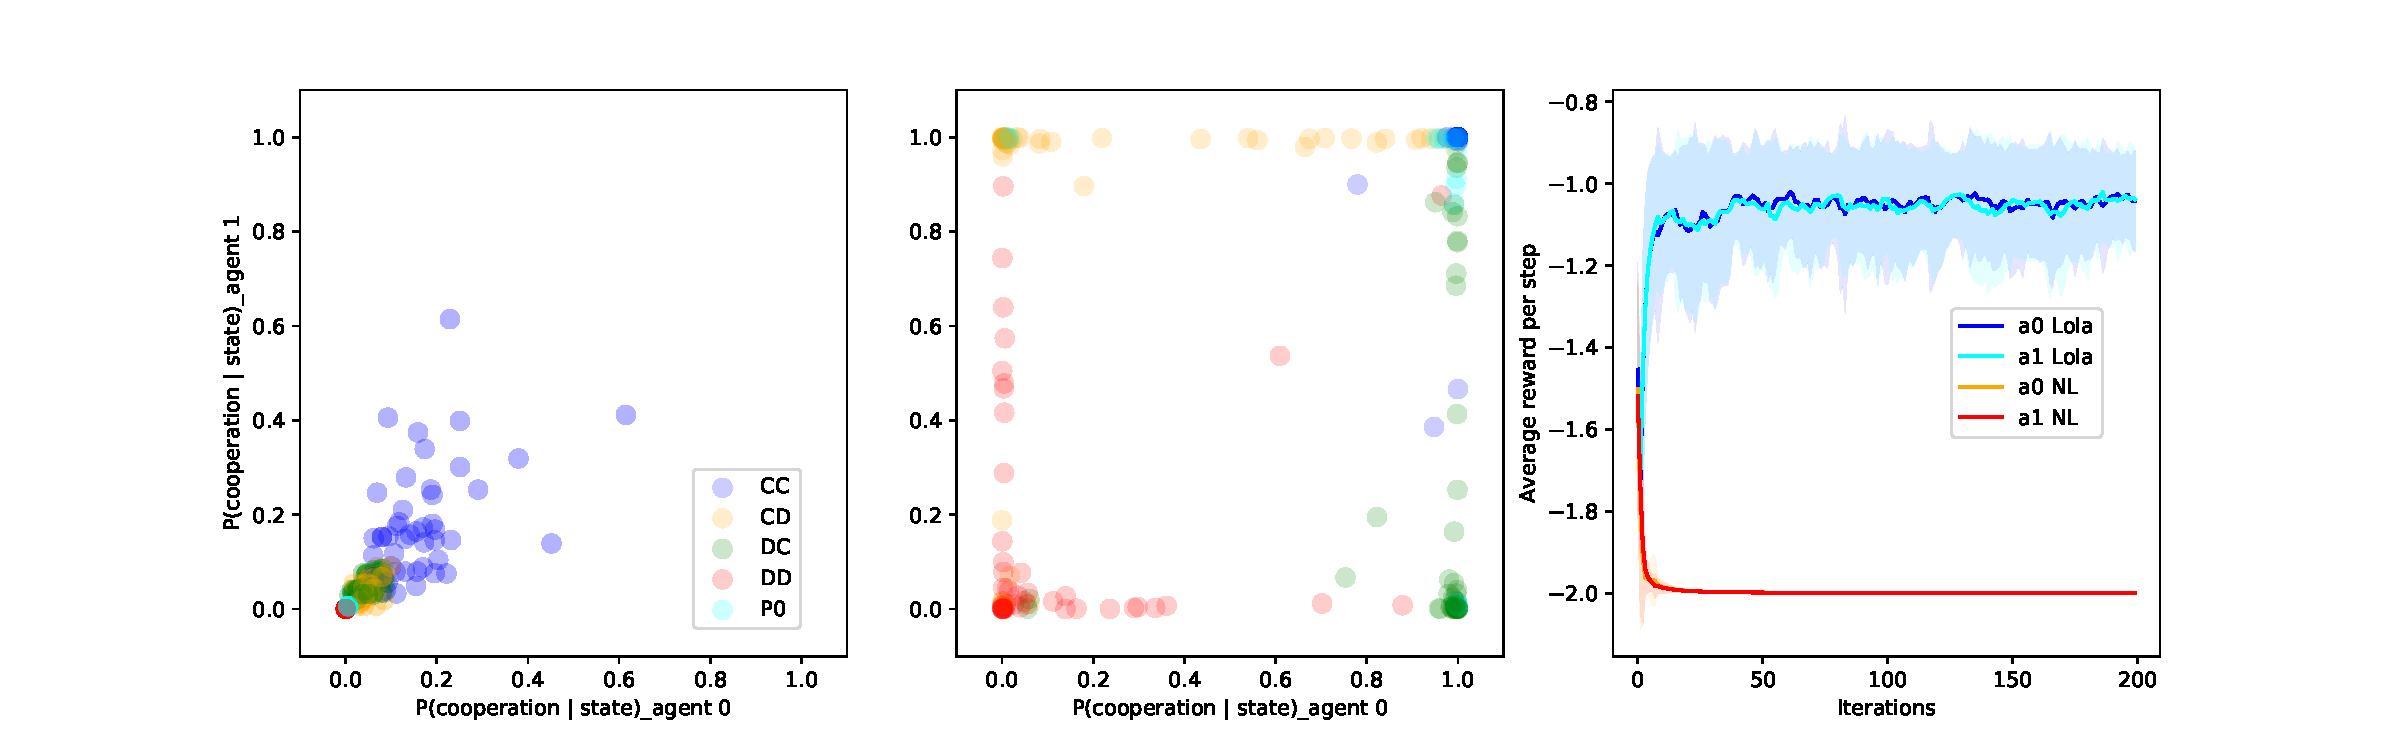
\includegraphics[width=1\textwidth]{figures/figure_1_prisoner}
	}
	\subfigure[]{
	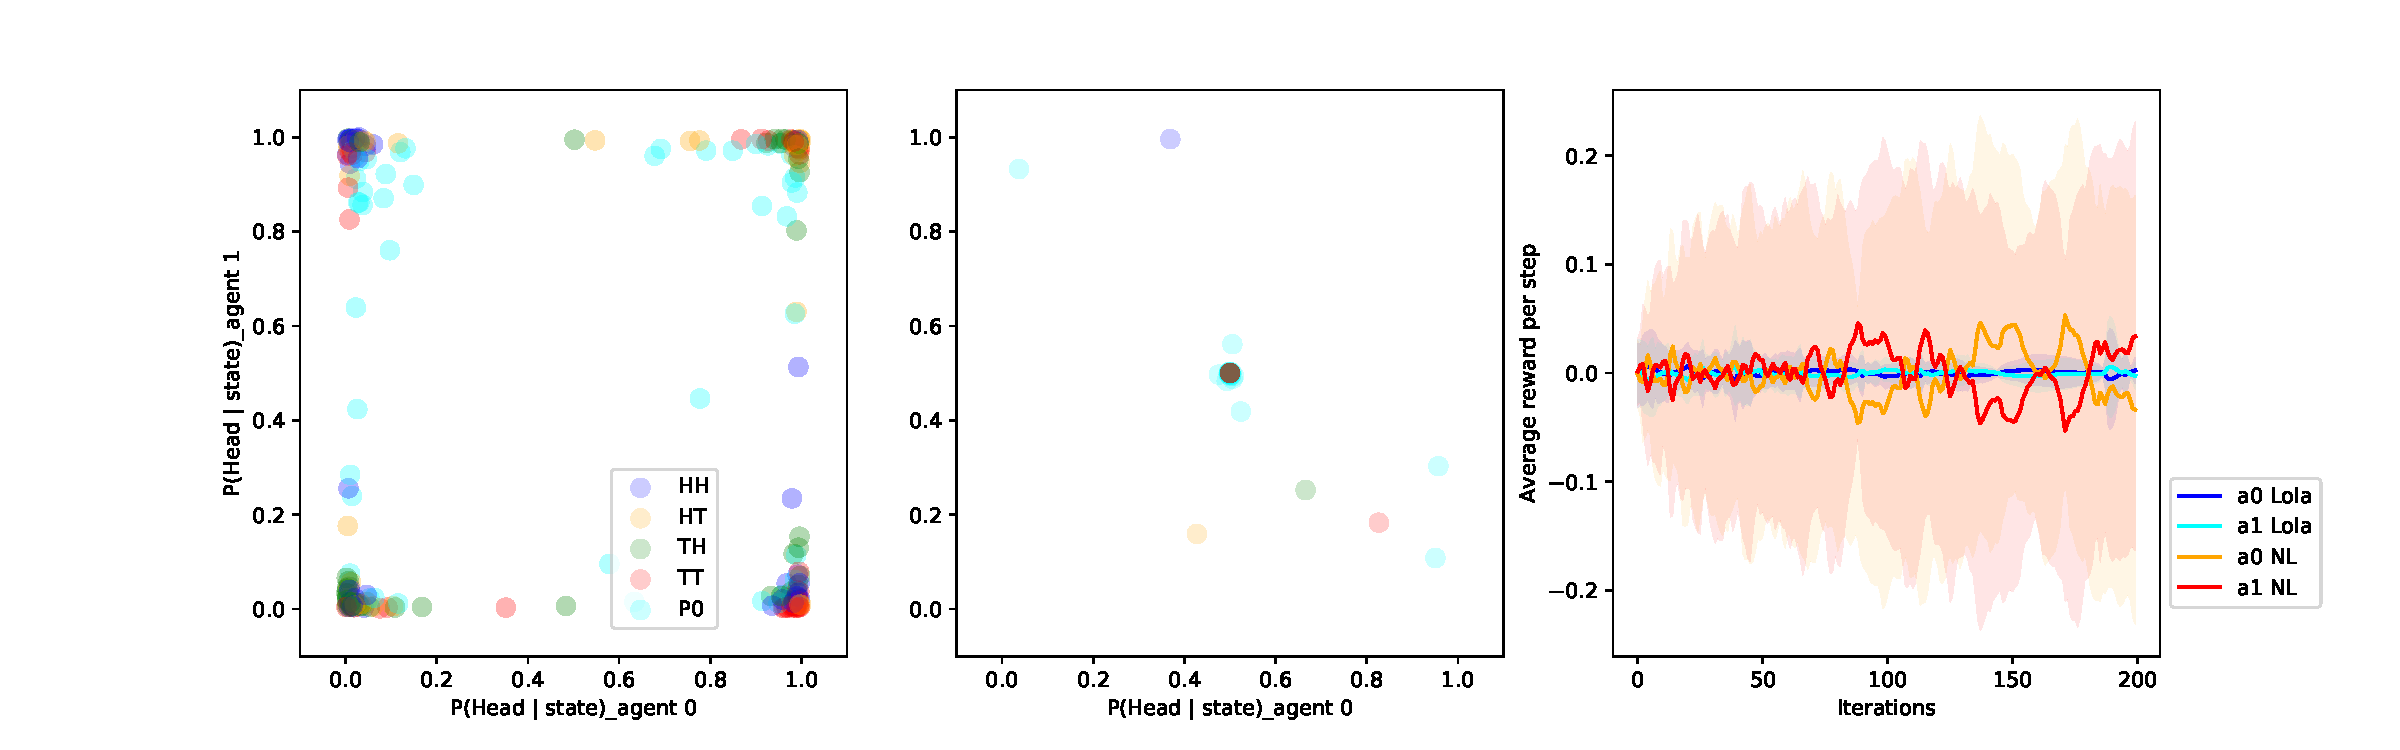
\includegraphics[width=1\textwidth]{figures/figure_1_coin}
	}
\label{fig:exact_V}
\caption{Shown is the probability of cooperation in the prisoners dilemma (a) and the probability of heads in the matching pennies game (b) at the end of 50 training runs for both agents as a function of state under naive learning (left) and LOLA (middle) when using the exact gradients of the value function. Also shown is the average return per step for naive and LOLA (right) }
\end{figure*}



\begin{figure*}[ht]
\centering
	\subfigure[]{
	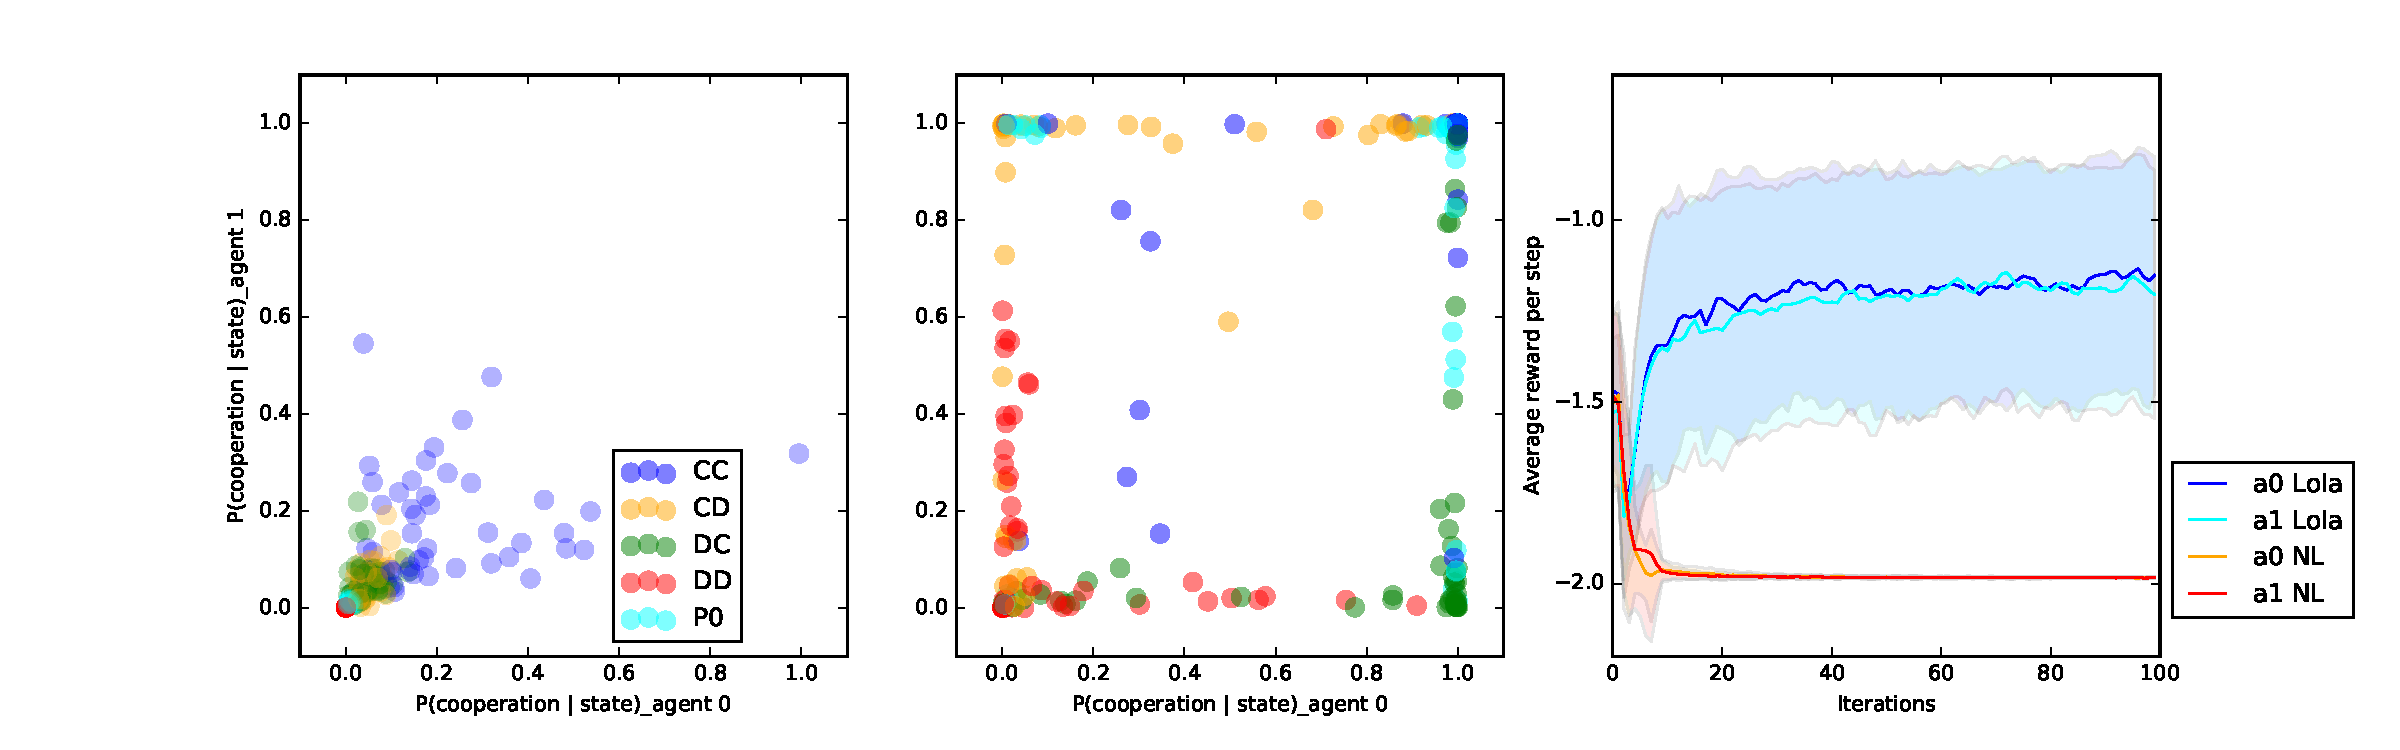
\includegraphics[width=1\textwidth]{figures/figure_1_prisoners_vr_c}
	}
	\subfigure[]{
	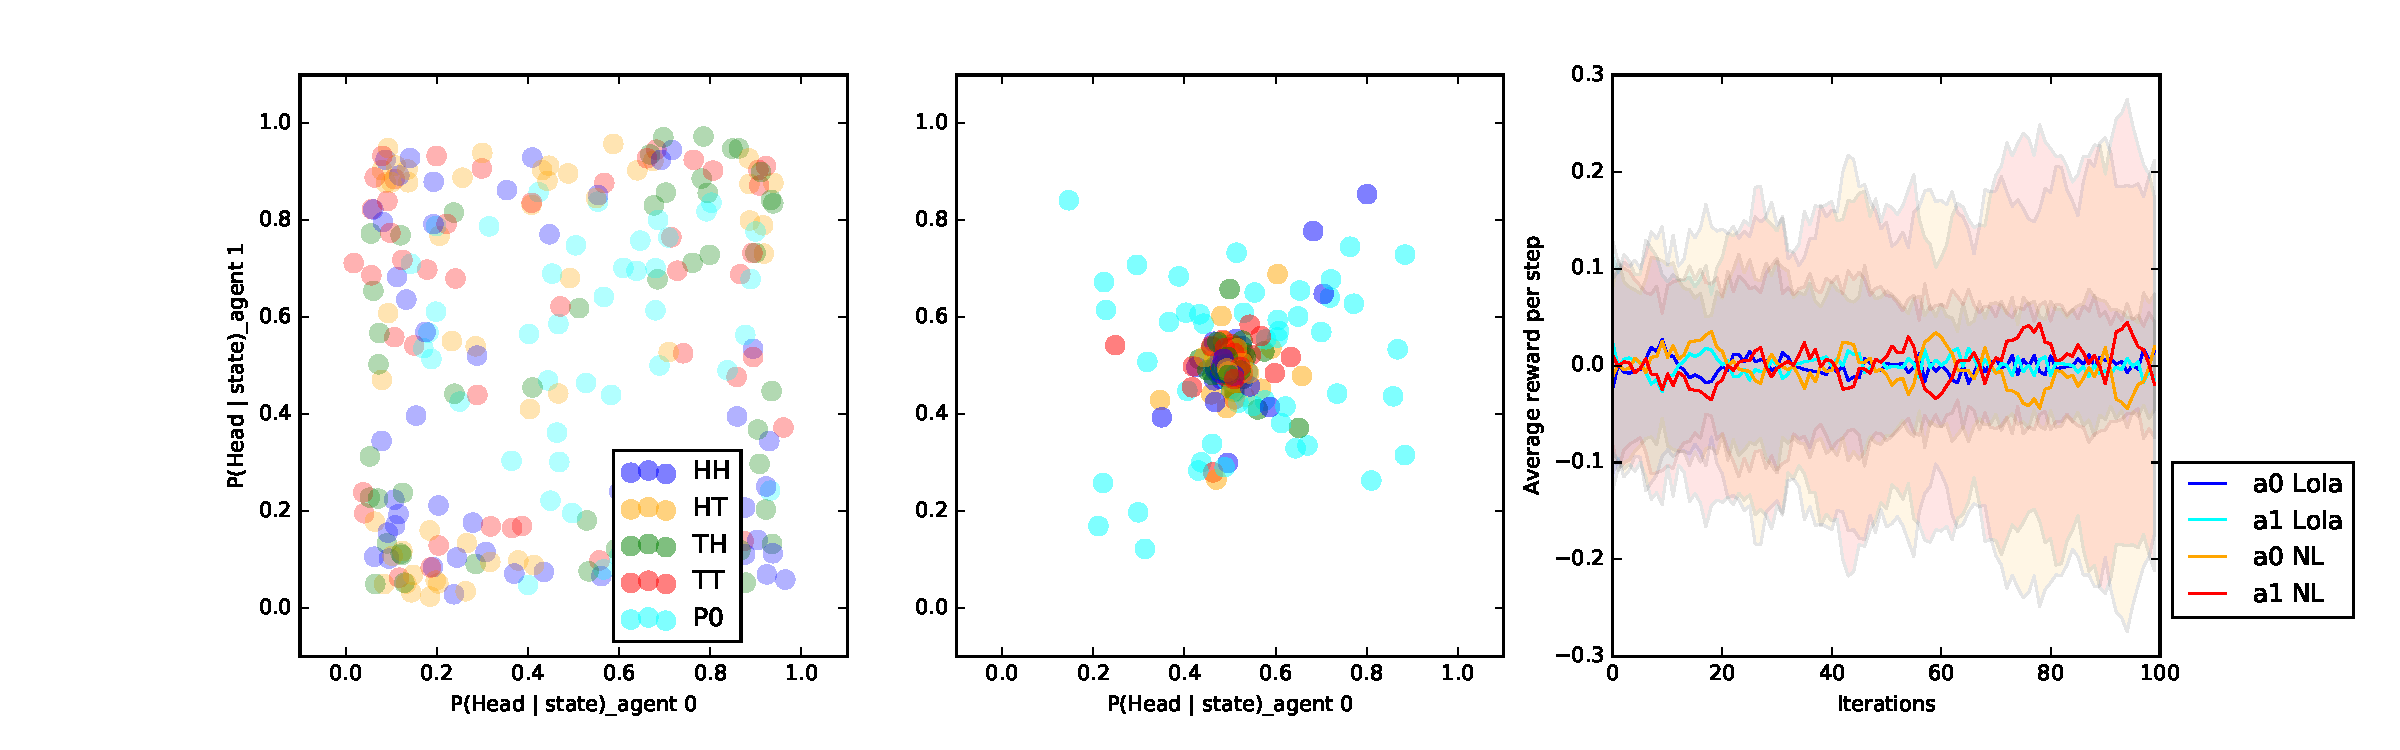
\includegraphics[width=1\textwidth]{figures/figure_1_pennies_vr_c}
	}
\label{fig:PG}
\caption{Same as Figure~\ref{fig:exact_V}, but using the policy gradient approximation for all terms. Clearly results are more noisy by qualitatively follow the results of the exact method.}
\end{figure*}
\end{document} 


